\section{Our Work}
The Travelex project approach at this moment was just a Proof of Concept (POC) with a 
few of testing locations where we are getting automatic notifications when an user 
is walking near there. The experiments were done in the TEC Campus Guadalajara area. \\

\begin{figure}[ht]
  \centering
  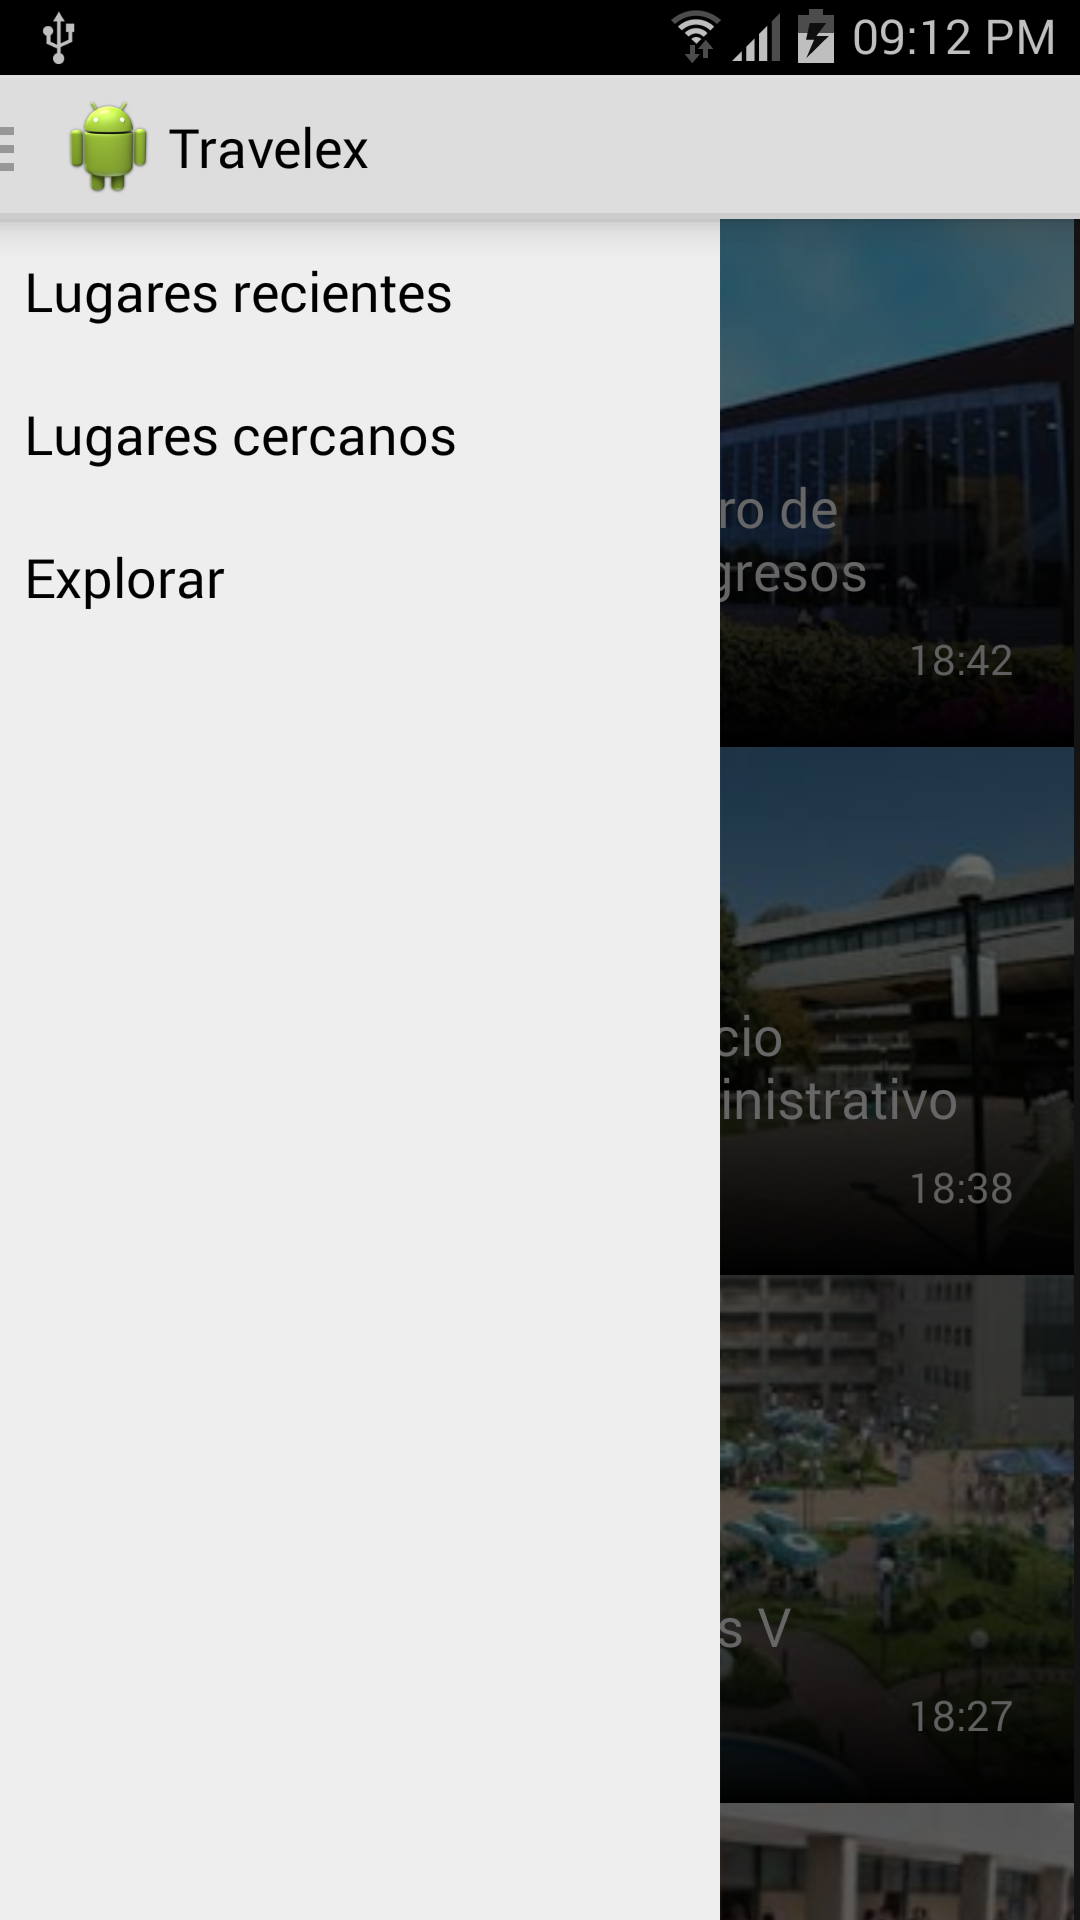
\includegraphics[scale=0.08]{travelex_menu}
  \caption{Travelex Main Menu View}
  \label{fig_menu}
\end{figure}

\subsection{Identifying places of Interest}
Based on the top 10 touristic places in Mexico shown in the TripAdvisor website[3]: \\

\begin{itemize}
  \item Playa del Carmen
  \item Puerto Vallarta
  \item Mexico City
  \item Cabo San Lucas
  \item Zihuatanejo
  \item Tulum
  \item Oaxaca
  \item San Miguel de Allende
  \item Puerto Escondido
  \item Acapulco
\end{itemize}

In order to provide the first proof of concept (POC), we started in our city; 
Guadalajara, which is also a  touristic city.

\begin{figure}[ht]
  \centering
  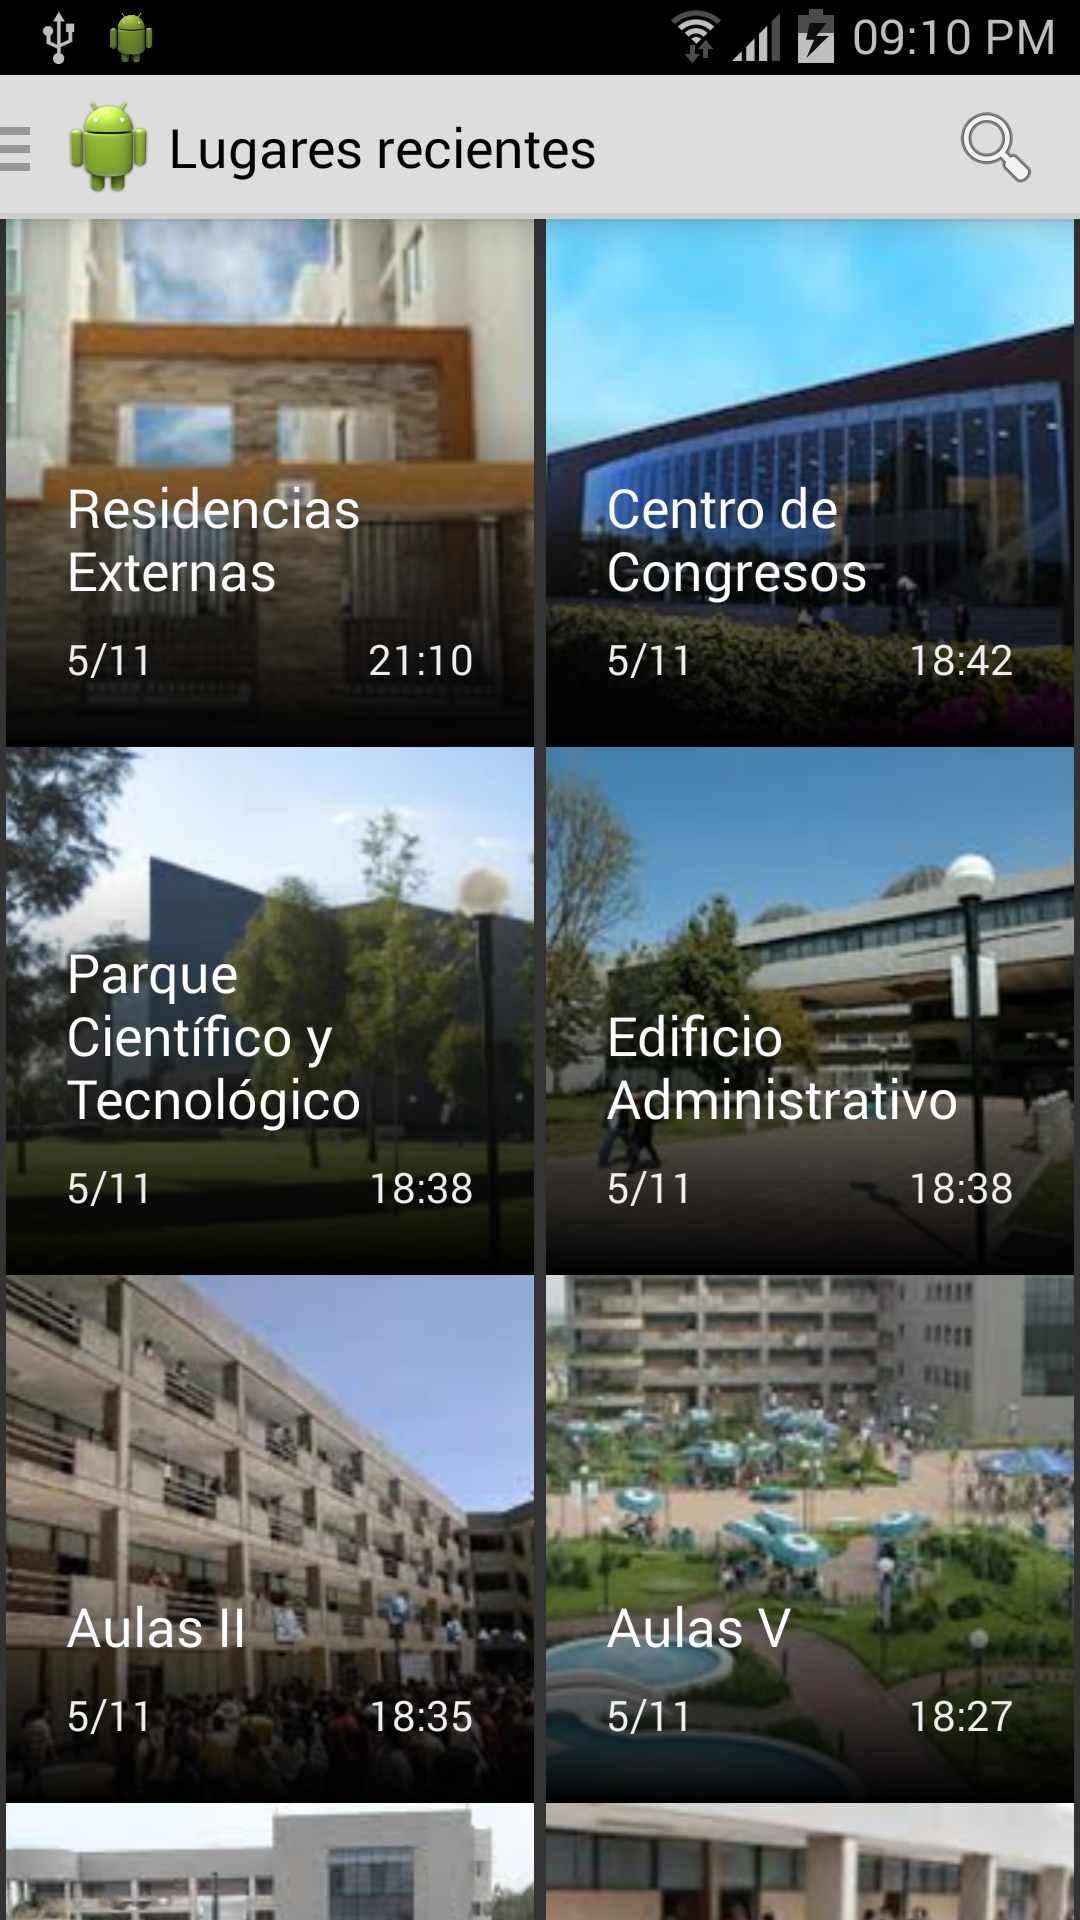
\includegraphics[scale=0.08]{travelex_places}
  \caption{Recent Places View}
  \label{fig_places}
\end{figure}

\begin{figure}[ht]
  \centering
  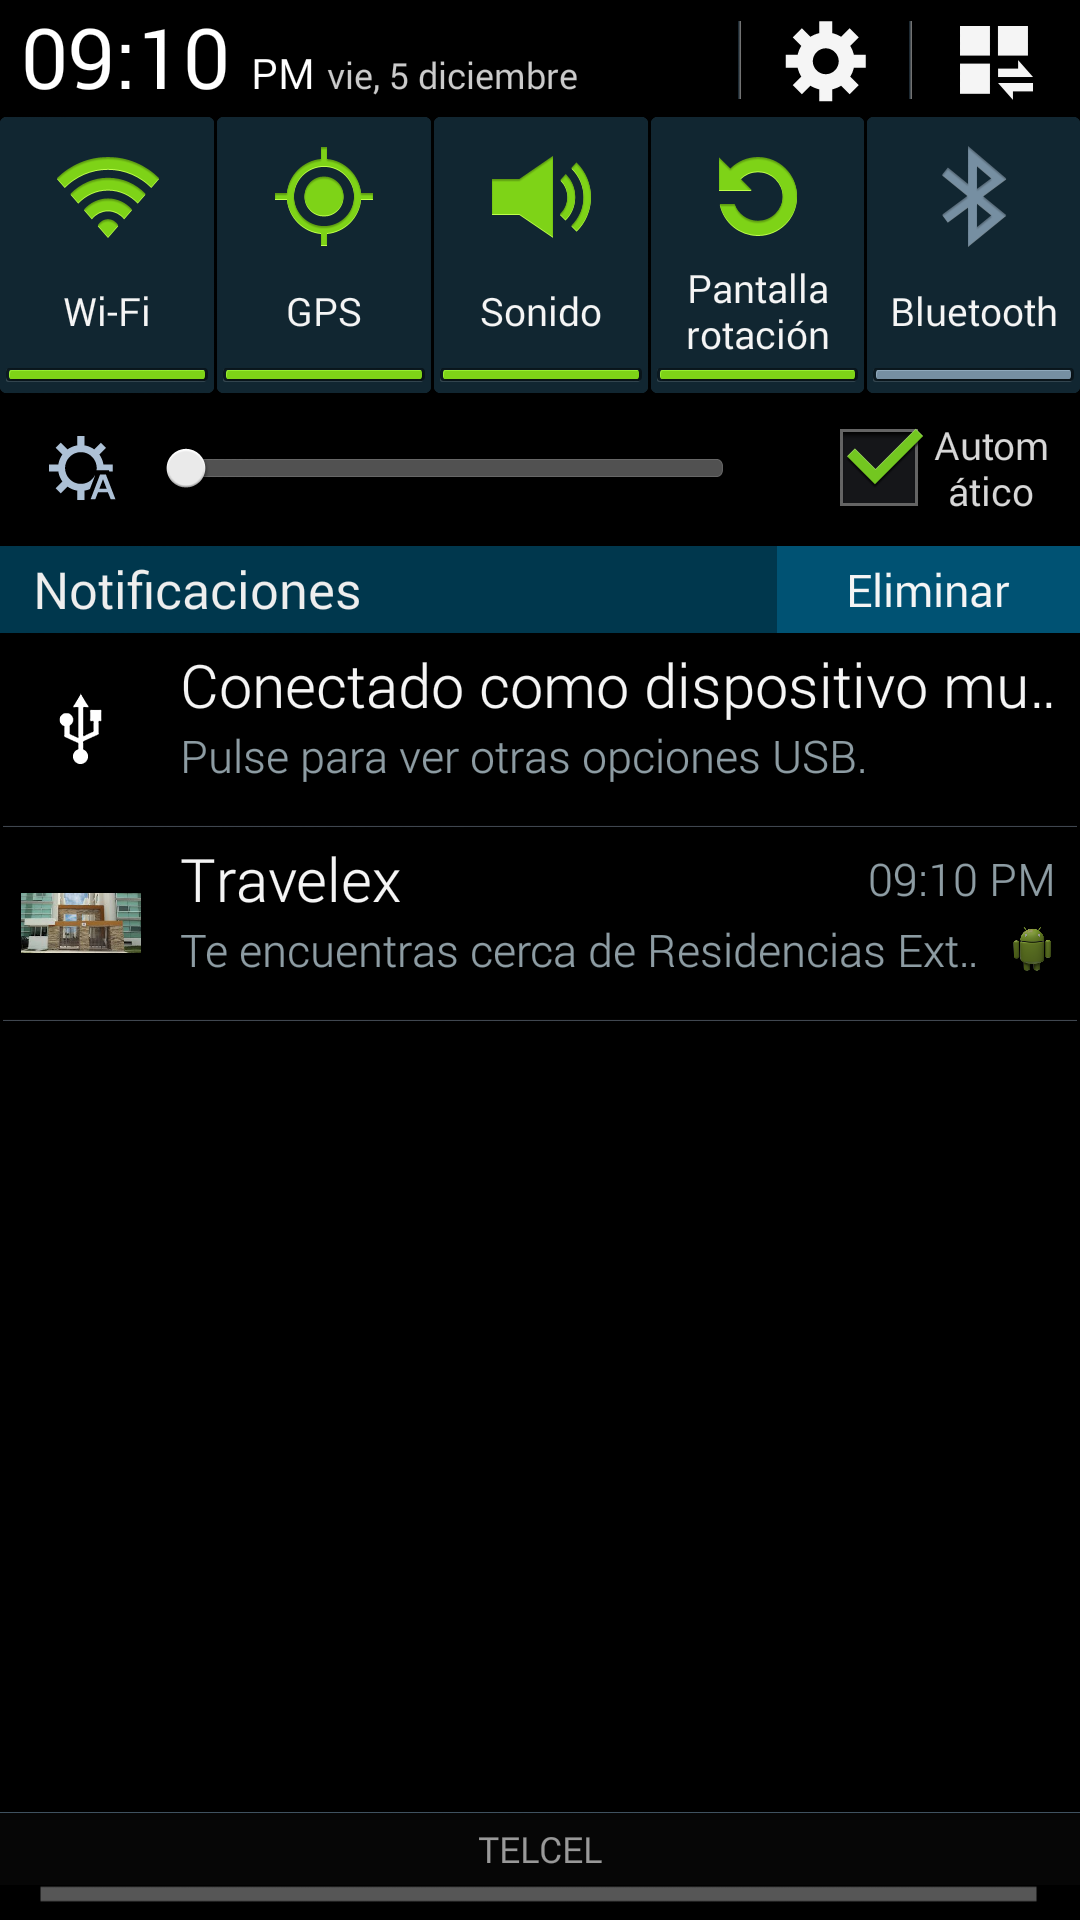
\includegraphics[scale=0.08]{travelex_notification}
  \caption{Recent Places View}
  \label{fig_notification}
\end{figure}

\subsection{Google Geofences Implementation}
A geofence defines a region of interest. For example, this may be a polygon outside of which a particular set of entities is not expected to stray. Geofences apply to particular collections.\\

Each geofence has a number of properties [4]:

\begin{itemize}
  \item ID: An opaque string used to refer to the geofence in calls to various methods. The ID for a geofence is assigned by the API at creation time. 

  \item Name: A user-defined string describing the geofence.

  \item Collection IDs: Zero or more IDs of collections to which the geofence applies. 

  \item Polygon: A polygon specifying the geofence's region. Crumbs recorded for entities belonging to one of the geofence's collections that fall within this polygon make the geofence active. This is required. 
\end{itemize}

For the  Travelex first approach the work-flow consists in the following 4 steps:\\

\begin{itemize}
  \item The application opens the  SQLite database file where it obtains the pre-defined GeoFences
  \item GeoFences information is sent to Google Geofencing API through a RESTFul API to be created and monitored
  \item A BroadcastReceiver service is started to receive transactions from Google API when it identifies when
        the users is near to a registered touristic place.
  \item The BroadcastReceiver service is started every time the phone is booted in order to let the Google API the phone's
        current location
\end{itemize}

\begin{figure}[ht]
  \centering
  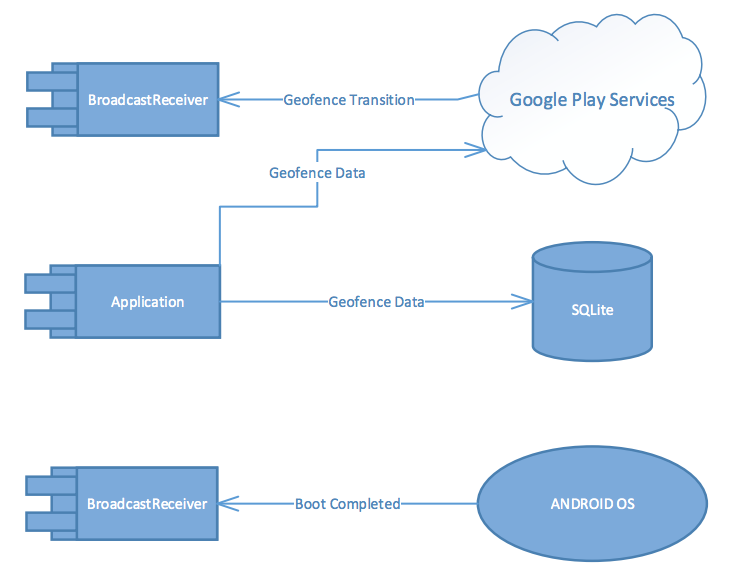
\includegraphics[width=2.5in]{travelex_flow}
  \caption{Travelex Data-Flow Diagram}
  \label{fig_sim}
\end{figure} 

NOTE: In our first testing approach, geofences were predefined and loaded at installation time in the SQLite 
database file.

\subsection{Project Schedule}

\subsubsection{Personnel Needs}
At the beginning of this project it can be started with a 10 people team, because it 
would start as a proof of concept for an specific city. Once the project get the 
accentance from the users, it will be escalated to more than 20 people where we will
have teams of developers, testers, designers, infrastructure operators and support.\\

Below are the number of human resources for the first release of the project:

\begin{itemize}
  \item 1 Software Architect
  \item 3 Android Developers
  \item 3 User Interface Designers
  \item 3 Testers 
\end{itemize}

\begin{figure}[ht]
  \centering
  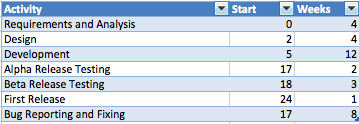
\includegraphics[width=2.5in]{schedule_table}
  \caption{Table of Project Schedule (on weeks)}
  \label{fig2}
\end{figure}


\begin{figure}[ht]
  \centering
  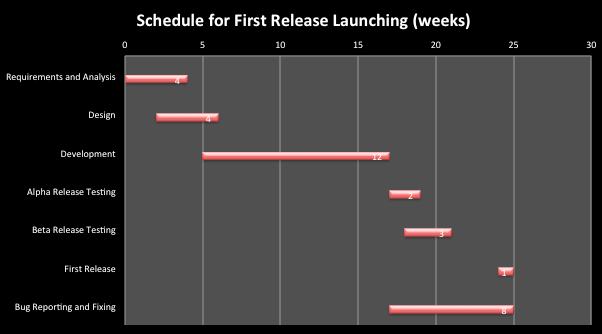
\includegraphics[width=2.5in]{schedule_gantt}
  \caption{Gantt Diagram of Project Schedule}
  \label{fig3}
\end{figure}

\subsection{Impact of the project}
The impact of this project can be separated in 2 principal beneficiary sectors:\\

1. Economic
  \begin{itemize}
    \item Local businesses get more tourists on their destinations
    \item More job opportunities due the demand of more services for tourists that are coming every vacation season
  \end{itemize}

2. Social 
\begin{itemize}
    \item Local culture is known around the world 
    \item Being role model in technology that is applied to improve the tourism
    \item Tourists will feel comfortable because there's a virtual assistant that will be there for directions to 
          amazing places to visit
\end{itemize}
